\documentclass{ximera}

\input{../preamble.tex}
\title[Prerequisite Videos: ]{Trigonometry: The Unit Circle}
\author{Ben Sencindiver}

\outcome{Understand how the unit circle is build and its meaning.}

\begin{document}
\begin{abstract}
  This series of videos will be aimed at using basic right angle trigonometry
  and the Pythagorean Theorem to develop an understanding of trigonometric
  functions and the unit circle and understand how it can be used and
  how what it means, as well some typical values on the unit circle
  and of trigonometric functions.
\end{abstract}
\maketitle

The following videos will cover the unit circle:

%% Introduction and Question 1
\textbf{Introduction and Question 1: The Pythagorean Theorem applications}
\begin{question}
%% Labeling this expandable option
\begin{flushright}
{\color{blue}(\emph{Click the arrow to the right to see the Introduction video and first question.})}
\end{flushright}
\begin{center}
\begin{expandable}
\youtube{df_2HysgT3k}
%% Multiple Choice Question 1
{\color{blue}(\emph{Click the arrow to the right to see the question
posed at the end of the video.})}
\begin{expandable}
If the hypotenuse of a right triangle is $8$cm long and one side is
$6$cm long, what is the length of the remaining side?
\begin{multipleChoice}
\choice{$1$}
\choice{$\sqrt{2}$}
\choice{$2$}
\choice{$\sqrt{14}$}
\choice[correct]{$2\sqrt{7}$}
\choice{$6$}
\choice{$8$}
\choice{$14$}
\choice{$28$}
\end{multipleChoice}
%% Hint
\begin{flushright}
{\color{blue}(\emph{Click the arrow to the right to see a hint.})}
\end{flushright}
\begin{expandable}
The Pythagorean theorem states that the square of the hypotenuse
of a right triangle is equal to the sum of the squares of the remaining
sides.
\end{expandable}
%% Example 1
\begin{flushright}
{\color{blue}(\emph{Click the arrow to the right to see an example.})}
\end{flushright}
\begin{expandable}
Example 1
\youtube{SjNxD9lswck}
\end{expandable}
\end{expandable}
\end{expandable}
\end{center}
\end{question}


%% Question 2
\textbf{Question 2: Defining trigonometric functions via right triangles}
\begin{question}
%% Labeling this expandable option
\begin{flushright}
{\color{blue}(\emph{Click the arrow to the right to see the definition
of trigonometric functions and second question.})}
\end{flushright}
\begin{center}
\begin{expandable}
\youtube{VCKoWgqH6qI}
%% Multiple Choice Question 2
{\color{blue}(\emph{Click the arrow to the right to see the question
posed at the end of the video.})}
\begin{expandable}
\begin{center}
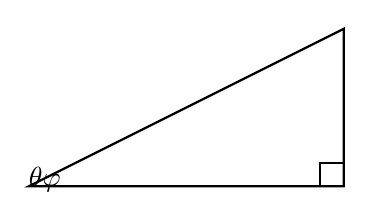
\begin{tikzpicture}[thick]
\coordinate (O) at (0,0);
\coordinate (A) at (4,0);
\coordinate (B) at (4,2);
\draw (O)--(A)--(B)--cycle;
%% The Right Angle
\coordinate (C) at (3.7,0);
\coordinate (D) at (3.7,0.3);
\coordinate (E) at (4,0.3);
\draw (C)--(D)--(E);
%% Line segment labeling
\tkzLabelSegment[below=2pt](O,A){b}
\tkzLabelSegment[above left=2pt](O,B){c}
\tkzLabelSegment[right=2pt](A,B){a}
%% Angle Labeling
\tkzMarkAngle[size=0.9cm,opacity=.4](A,O,B)
\tkzLabelAngle[pos = 0.7](A,O,B){$\theta$}
%% Angle Labeling
\tkzMarkAngle[size=0.65cm, opacity=.4](O,B,A)
\tkzLabelAngle[pos = 0.45](O,B,A){$\varphi$}
\end{tikzpicture}
\end{center}
Consider the triangle below where $a = 6$, $b=2\sqrt{7}$,
and $c=8$. What is $\sin( \theta)$?\\
\begin{prompt}
\[
\sin(\theta)\text{ is }\answer[given]{6/8}
\]
\end{prompt}
%% Refresher 2
\begin{flushright}
{\color{blue}(\emph{Click the arrow to the right to see a short refresher.})}
\end{flushright}
\begin{expandable}
Refresher 2
\youtube{fRLXoOJzkv4}
\end{expandable}
%% Example 2
\begin{flushright}
{\color{blue}(\emph{Click the arrow to the right to see an example.})}
\end{flushright}
\begin{expandable}
Example 2
\youtube{sJTixDB9W7c}
\end{expandable}
\end{expandable}
\end{expandable}
\end{center}
\end{question}


%% Question 3
\textbf{Question 3: What is a radian and converting between radians and degrees}
\begin{question}
%% Labeling this expandable option
\begin{flushright}
{\color{blue}(\emph{Click the arrow to the right to see the video about radians, converting between radians and degrees, and the third question.})}
\end{flushright}
\begin{center}
\begin{expandable}
\youtube{JTqB-ixAf3o}
%% Multiple Choice Question 3
{\color{blue}(\emph{Click the arrow to the right to see the answers 
to the question posed at the end of the video.})}
\begin{expandable}
What is $35^\circ$ in radians?
\begin{prompt}
\[
35^\circ\text{ in radians is }\answer[given]{35 \pi / 180}
\]
\end{prompt}
%% Refresher 3
\begin{flushright}
{\color{blue}(\emph{Click the arrow to the right to see a short refresher.})}
\end{flushright}
\begin{expandable}
Refresher 3
\youtube{n8lMuOdrXUk}
\end{expandable}
%% Example 3
\begin{flushright}
{\color{blue}(\emph{Click the arrow to the right to see an example.})}
\end{flushright}
\begin{expandable}
Example 3
\youtube{CVIvPvgvZ5g}
\end{expandable}
\end{expandable}
\end{expandable}
\end{center}
\end{question}


%% Question 4
\textbf{Question 4: Evaluating trigonometric functions
without a triangle}
\begin{question}
%% Labeling this expandable option
\begin{flushright}
{\color{blue}(\emph{Click the arrow to the right to see the video about
radians, converting between radians and degrees, and the fourth question.})}
\end{flushright}
\begin{center}
\begin{expandable}
\youtube{JTqB-ixAf3o}
%% Multiple Choice Question 4
{\color{blue}(\emph{Click the arrow to the right to see the  question
posed at the end of the video.})}
\begin{expandable}
What is $\tan\Big(\frac{\pi}{4}\Big)$?
\begin{prompt}
\[
\tan\Big(\frac{\pi}{4}\Big)\text{ is }\answer[given]{1}
\]
\end{prompt}
%% Example 4
\begin{flushright}
{\color{blue}(\emph{Click the arrow to the right to see an example.})}
\end{flushright}
\begin{expandable}
Example 4
\youtube{vH1YcPlTqXw}
\end{expandable}
\end{expandable}
\end{expandable}
\end{center}
\end{question}


%% Question 5
\textbf{Question 5: Building the unit circle in the first quadrant and understanding it}
\begin{question}
%% Labeling this expandable option
\begin{flushright}
{\color{blue}(\emph{Click the arrow to the right to see
the
video about how to build the unit circle, what points
on the
unit circle mean, and the fifth question.})}
\end{flushright}
\begin{center}
\begin{expandable}
\youtube{ZxKCQczwzbg}
%% Multiple Choice Question 5
{\color{blue}(\emph{Click the arrow to the right to see the question
posed at the end of the video.})}
\begin{expandable}
In the first quadrant, how many solutions are there to $\cos(\theta) = \frac{\pi}{2}$
\begin{prompt}
\[
\text{ There are }\answer[given]{0}\text{ solution(s)
to }\cos(\theta)=\frac{\pi}{2}\text{ in the first quadrant.}
\]
\end{prompt}
%% Refresher 5
\begin{flushright}
{\color{blue}(\emph{Click the arrow to the right to see a short refresher.})}
\end{flushright}
\begin{expandable}
Refresher 5
\youtube{CwFNvNp38bM}
\end{expandable}
%% Example 5
\begin{flushright}
{\color{blue}(\emph{Click the arrow to the right to see an example.})}
\end{flushright}
\begin{expandable}
Example 5
\youtube{nB7FXsPx1kI}
\end{expandable}
\end{expandable}
\end{expandable}
\end{center}
\end{question}


%% Question 6
\textbf{Question 6: Extending the unit circle and trigonometric
functions to all angles}
\begin{question}
%% Labeling this expandable option
\begin{flushright}
{\color{blue}(\emph{Click the arrow to the right to see the
video about extending the unit circle trigonometric functions to all
angles, and the sixth question.})}
\end{flushright}
\begin{center}
\begin{expandable}
\youtube{uF7wSNToPwU}
%% Multiple Choice Question 6
{\color{blue}(\emph{Click the arrow to the right to see the question
posed at the end of the video.})}
\begin{expandable}
What is $\csc\Big(\dfrac{4\pi}{3}\Big)$?
\begin{prompt}
\[
\csc\Big( \dfrac{4\pi}{3}\Big) \text{ is equal to } \answer[given]{-\frac{2}{\sqrt(3)}}.
\]
\end{prompt}
%% Refresher 6
\begin{flushright}
{\color{blue}(\emph{Click the arrow to the right to see a short refresher.})}
\end{flushright}
\begin{expandable}
Refresher 6
\youtube{QiBZufrEhC8}
\end{expandable}
%% Example 6
\begin{flushright}
{\color{blue}(\emph{Click the arrow to the right to see an example.})}
\end{flushright}
\begin{expandable}
Example 6
\youtube{i0gPEAqd5eg}
\end{expandable}
\end{expandable}
\end{expandable}
\end{center}
\end{question}



%% Question 7
\textbf{Question 7: The First Pythagorean Identity and the Unit Circle}
\begin{question}
%% Labeling this expandable option
\begin{flushright}
{\color{blue}(\emph{Click the arrow to the right to see the
video about the first Pythagorean Identity, and the seventh question.})}
\end{flushright}
\begin{center}
\begin{expandable}
\youtube{BbcPyRsYoSs}
%% Multiple Choice Question 7
{\color{blue}(\emph{Click the arrow to the right to see the question
posed at the end of the video.})}
\begin{expandable}
What is the resulting identity if both sides of the Pythagorean Identity are multiplied by $\csc^2(\theta)$? (Please simplify any products or division of trigonometric functions to one trigonometric function if possible)
\begin{prompt}
\[
1 + \answer[given]{\cot^2(\theta)} \hspace{1cm} = \answer[given]{\csc^2(\theta)}.
\]
\end{prompt}
%% Example 7
\begin{flushright}
{\color{blue}(\emph{Click the arrow to the right to see an example.})}
\end{flushright}
\begin{expandable}
Example 7
\youtube{tOe_ZgYlgJM}
\end{expandable}
\end{expandable}
\end{expandable}
\end{center}
\end{question}



%% Question 8
\textbf{Question 8: Domains of Pythagorean Identities}
\begin{question}
%% Labeling this expandable option
\begin{flushright}
{\color{blue}(\emph{Click the arrow to the right to see the
video 
about domains of Pythagorean Identities, and the eighth question.})}
\end{flushright}
\begin{center}
\begin{expandable}
\youtube{useamk-mVuc}
%% Multiple Choice Question 8
{\color{blue}(\emph{Click the arrow to the right to see the question
posed at the end of the video.})}
\begin{expandable}
For what values of $\theta$ is it true that $1 + \cot^2(\theta) = \csc^2(\theta)$?

\begin{multipleChoice}
\choice{For all values of $\theta$.}
\choice{For all values of $\theta$, except $0$.}
\choice{For all values of $\theta$, except $\frac{\pi}{2}$.}
\choice[correct]{For all values of $\theta$, except $\pi n$ when $n$ is an integer.}
\choice{For all values of $\theta$, except $2\pi n$ when $n$ is an integer.}
\choice{For all values of $\theta$, except $\frac{\pi}{2} +  \pi n$ when $n$ is an integer.}
\choice{For all values of $\theta$, except $\frac{\pi}{2} +  2\pi n$ when $n$ is an integer.}
\end{multipleChoice}
%% Example 8
\begin{flushright}
{\color{blue}(\emph{Click the arrow to the right to see an example.})}
\end{flushright}
\begin{expandable}
Example 8
\youtube{-Ys2XHhZ1FQ}
\end{expandable}
\end{expandable}
\end{expandable}
\end{center}
\end{question}




\end{document}
